\IfFileExists{../../_preamble/check_file.tex}% prüfen aus welcher datei der aufruf stattfindet
{%
\providecommand{\myPath}{../../}% file exists=true: befinde mich im unterverzeichnis
}%
{%
\providecommand{\myPath}{}% file exists=false: befinde mich im root_verzeichnis
}%
\documentclass[tikz]{standalone}
%% läd standalone-klasse mit tikz-argument
%//Tikzbibliotheken\\%
\usetikzlibrary{						% Bibliotheken zur direkten Einbindung in TIKZEdt
arrows, 
fit,
shapes.geometric, 
matrix,
calc,
decorations.markings,
decorations.pathreplacing,
decorations.pathmorphing,
backgrounds,
shadings, 
shadows,
positioning,
mindmap,
trees,
datavisualization
}%% diverse tikz-bibliotheken
%%Font etc.%%
\usepackage{lmodern}					% OK, Latin Modern font,											check: 25.08.18
\usepackage{xcolor} 					% OK, Definieren und Nutzen von versch. Farben						check: 25.08.18
\usepackage{graphicx}					% OK, Bereitstellen von \includegraphics							check: 25.08.18

%%Forest%%
\usepackage{forest}						% OK, Baumdarstellung aus dem linguistischen Bereich				check: 25.08.18
\useforestlibrary{edges}

%%Venndiagramm%%
\usepackage{venndiagram}				% OK, Definieren und Darstellen von Venndiagrammen					check: 25.08.18

%%Tabellen%%
\usepackage{booktabs}					% OK, Schönere Tabellen ohne vertikale Linien \toprule etc.			check: 25.08.18
\usepackage{tabularx}					% OK, Weiterer Spaltentyp passt Tabellenbreite  automatisch an		check: 25.08.18
\usepackage{multirow}					% OK, Zellenspannung über mehrere Zeilen							check: 25.08.18
%\usepackage{makecell}					% OK, Tabellenlayout (Tabaellenheader) ähnlich \multirow			check: 25.08.18
\usepackage{tablefootnote}				% OK, Fußnoten in Tabellen (\footnote funktioniert nicht)			check: 25.08.18
\usepackage{array} 						% OK, Erstellen eigener Columntypen in Tabellenumgebungen			check: 25.08.18

%%Grafiken und Plots%%
\usepackage{tikz} 						% OK, Natives zeichnen in Latex ,									check: 25.08.18
\usepackage{tikz-cd} 					% OK, Erstellen von kommutativen Diagrammen in Tikz,				check: 25.08.18
\usepackage{pgfplots}					% OK, Plotten von Daten,											check: 25.08.18
\pgfplotsset{compat=newest}				% OK, Einstellen der Kompatibilitätsversion,						check: 25.08.18
\usepackage{pgfplotstable}				% OK, Plotten und schreiben von Daten in Tabellen,					check: 25.08.18
\usepackage{pgfcalendar} 				% OK, Umrechnen von Datumskoordinaten,								check: 25.08.18
\usepgfplotslibrary{dateplot}			% OK, Plotten von Datumskoordinaten,								check: 25.08.18
\usepgfplotslibrary{units}				% OK, Darstellen von Einheiten als Achsenlabel,						check: 25.08.18%% nur laden wenn weitere graphic pakete benötigt werden (tabellen, pgfplot,...)
%%define tikz-stlyes here, colours etc.
\tikzset{
block_phantom/.style={block_normal, draw=red, fill=none},
block_phantom/.style={block_normal, draw=blue, fill=none}
}
%\tikzstyle{block_phantom}=[block_normal, draw=red, fill=none]%% tikz-styles, farben etc.
\begin{document}%
\IfFileExists{../../_preamble/check_file.tex}% prüfen aus welcher datei der aufruf stattfindet
{%file exists=true: befinde mich im unterverzeichnis
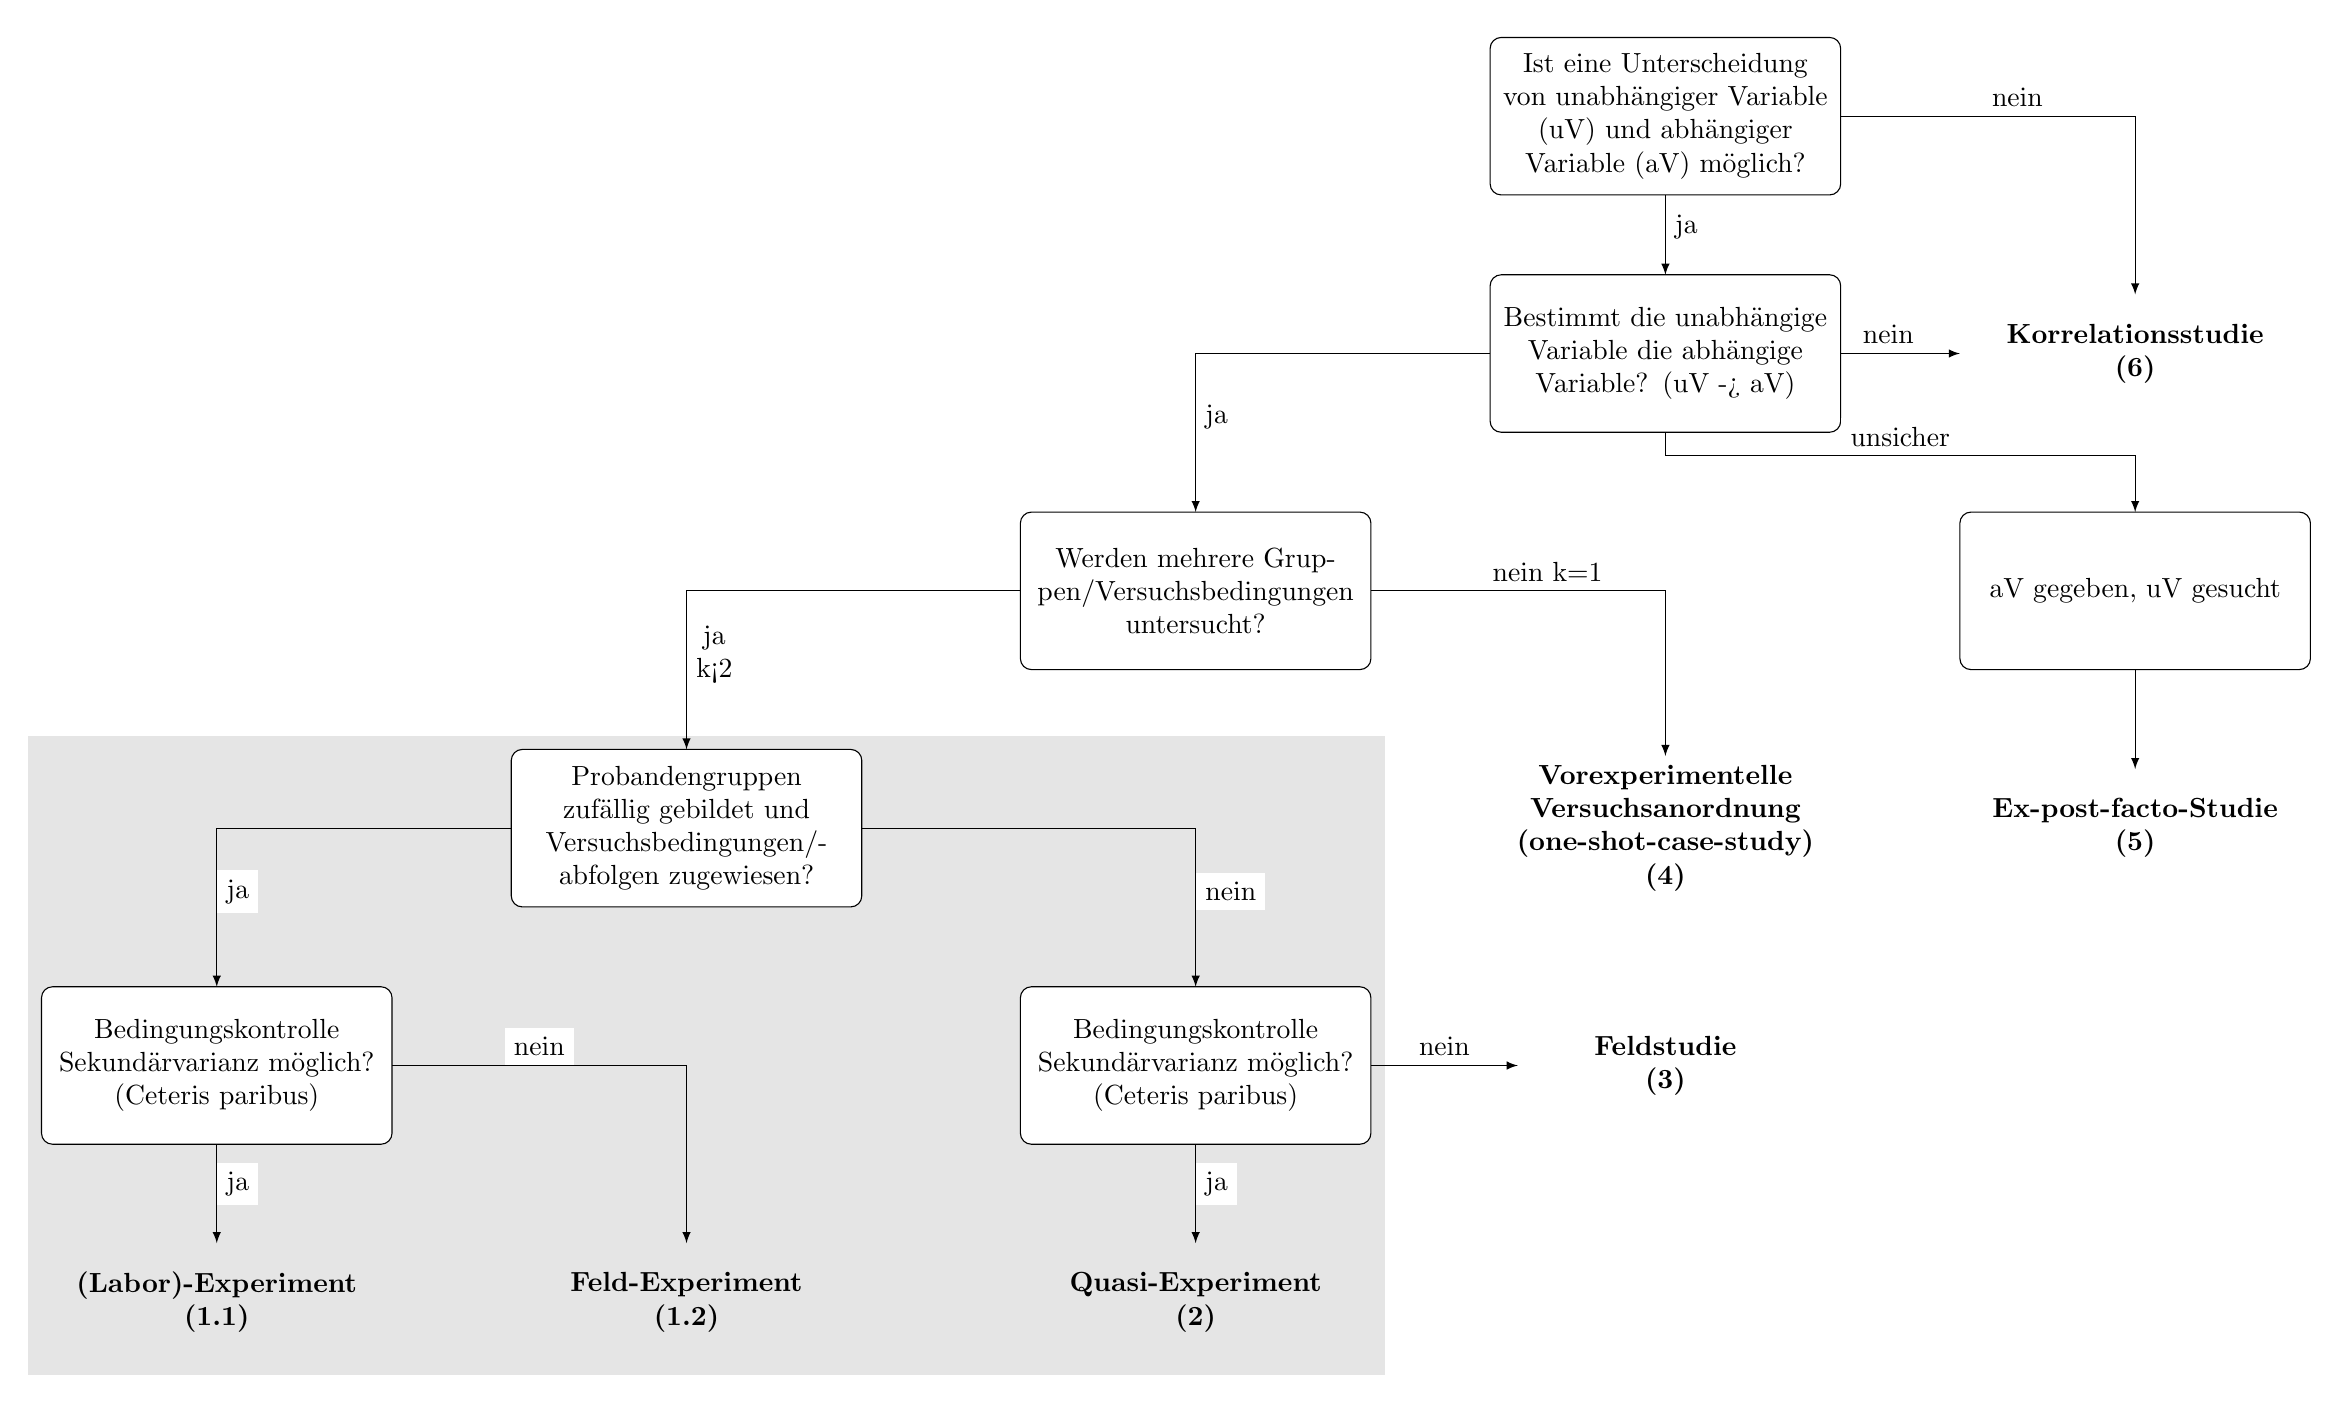
\begin{tikzpicture}
[auto,
decision/.style={diamond, draw=blue, thick, fill=blue!20,text width=4.5em,align=flush center,inner sep=1pt},
block/.style ={ rectangle, draw, fill=white,  text centered, minimum height=15mm, text width=12em},
block_todo/.style ={ rectangle, draw, fill=white,  text centered, minimum height=15mm, text width=12em, rounded corners, outer sep=5},
block_done/.style ={ rectangle, draw, fill=white,  text centered, minimum height=15mm, text width=12em, rounded corners, outer sep=5},
block_normal/.style ={ rectangle, draw, fill=white,  text centered, minimum height=2cm, text width=12em, rounded corners, outer sep=0},
block_exp/.style ={ rectangle, draw=none, fill=none,  text centered, minimum height=1.5cm, text width=12em,font=\bfseries, rounded corners, outer sep=0},
block_phantom/.style ={ block_normal, draw=none, fill=none},
block_background/.style ={ rectangle,  draw=none, fill=black,  text centered, minimum height=15mm,fill opacity=.1, rounded corners=0, inner sep=5},
output/.style ={trapezium,draw,fill=none, minimum height=10mm,  align=center, trapezium left angle=60, trapezium right angle=120, text width=50},
line_inner/.style ={draw, -latex,shorten >=0pt, shorten <=0pt},
kreis/.style ={ circle, draw, fill=white,  text centered, minimum height=15mm, text width=10em, rounded corners, outer sep=0, minimum size=.4cm},
zylinder/.style={cylinder, draw, fill=yellow!20,shape border rotate=90, text height=5, align=center, aspect=.1, text width=10em, minimum height=6.5em, minimum width=2em},
line_outer/.style ={draw, -latex,shorten >=4pt, shorten <=4pt}]
]


\matrix (table) [column sep=1.5cm,row sep=1cm, ampersand replacement=\&,  nodes in empty cells, in front of path]
{
% row 1
\node [block_phantom] (11) {};  \& [0cm]
\node [block_phantom] (12) {}; \& [.5cm]
\node [block_phantom] (13) {};\&
\node [block_normal] (14) {Ist eine Unterscheidung von unabh\"angiger Variable (uV) und abh\"angiger Variable (aV) m\"oglich?};\&
\node [block_phantom] (15) {};\\
 % row 2
\node [block_phantom] (21) {};\& 
\node [block_phantom] (22) {}; \&
\node [block_phantom] (23) {};\&
\node [block_normal] (24) {Bestimmt die unabh\"angige Variable die abh\"angige Variable? (uV -> aV)};\&
\node [block_exp] (25) {Korrelationsstudie \\(6)}; \\
 % row 3
\node [block_phantom] (31) {};\& 
\node [block_phantom] (32) {}; \&
\node [block_normal] (33) {Werden mehrere Gruppen/Versuchsbedingungen untersucht?};\&
\node [block_phantom] (34) {};\&
\node [block_normal] (35) {aV gegeben, uV gesucht}; 
  \\
 % row 4
\node [block_phantom] (41) {};\& 
\node [block_normal] (42) {Probandengruppen zuf\"allig gebildet  und  Versuchsbedingungen/-abfolgen zugewiesen?}; \&
\node [block_phantom] (43) {};\&
\node [block_exp] (44) {Vorexperimentelle Versuchsanordnung (one-shot-case-study)\\(4)};\&
\node [block_exp] (45) {Ex-post-facto-Studie\\(5)};  
   \\
 % row 5
\node [block_normal] (51) {Bedingungskontrolle Sekund\"arvarianz m\"oglich? (Ceteris paribus)};\& 
\node [block_phantom] (52) {}; \&
\node [block_normal] (53) {Bedingungskontrolle Sekund\"arvarianz m\"oglich? (Ceteris paribus)};\&
\node [block_exp,text width=10em] (54) {Feldstudie \\(3)};\&
\node [block_phantom] (55) {}; \\
  % row 6
\node [block_exp] (61) {(Labor)-Experiment\\(1.1)};\& 
\node [block_exp] (62) {Feld-Experiment\\(1.2)}; \&
\node [block_exp] (63) {Quasi-Experiment\\(2)};\&
\node [block_phantom] (64) {};\&
\node [block_phantom] (65) {}; \\
};

%%Pfeile%%%
\draw[line_inner] (14.south) -|  ++(0,0) -|  node[pos=.7, fill=white, rotate=0, align=center] {ja}(24.north);
\draw[line_inner] (24.west) -|  ++(0,0) -|  node[pos=.7,fill=white , rotate=0, align=center] {ja}(33.north);
\draw[line_inner] (33.west) -|  ++(0,0) -|  node[fill=white, pos=.7, rotate=0, align=center] {ja\\k<2}(42.north);
\draw[line_inner] (42.west) -|  ++(0,0) -|  node[fill=white, pos=.7, rotate=0, align=center] {ja}(51.north);
\draw[line_inner] (51.east) -|  ++(0,0) -|  node[fill=white, pos=.25, rotate=0, align=center] {nein}(62.north);
\draw[line_inner] (51.south) -|  ++(0,0) -|  node[fill=white, pos=.7, rotate=0, align=center] {ja}(61.north);
\draw[line_inner] (53.south) -|  ++(0,0) -|  node[fill=white, pos=.7, rotate=0, align=center] {ja}(63.north);
\draw[line_inner] (42.east) -|  ++(0,0) -|  node[fill=white, pos=.7, rotate=0, align=center] {nein}(53.north);
\draw[line_inner] (33.east) -|  ++(0,0) -|  node[fill=white, pos=.3, rotate=0, align=center] {nein k=1}(44.north);
\draw[line_inner] (53.east) -|  ++(0,0) |-  node[fill=white, pos=.75, rotate=0, align=center] {nein}(54.west);
\draw[line_inner] (14.east) -|  ++(0,0) -|  node[fill=white, pos=.3, rotate=0, align=center] {nein}(25.north);
\draw[line_inner] (24.east) -|  ++(0,0) |-  node[fill=white, pos=.7, rotate=0, align=center] {nein}(25.west);
\draw[line_inner] (24.south) -|  ++(0,-.3) -|  node[fill=white, pos=.25, rotate=0, align=center] {unsicher}(35.north);
\draw[line_inner] (35.south) -|  ++(0,-.4) -|  node[ pos=.3, rotate=0, align=center] {}(45.north);

%%%Background%%%%
\begin{scope}[on background layer]
\node[fit=(41)(63), block_background]{};
\end{scope}
%%%Background%%%%


\end{tikzpicture}%
}%
{%file exists=false: befinde mich im root_verzeichnis
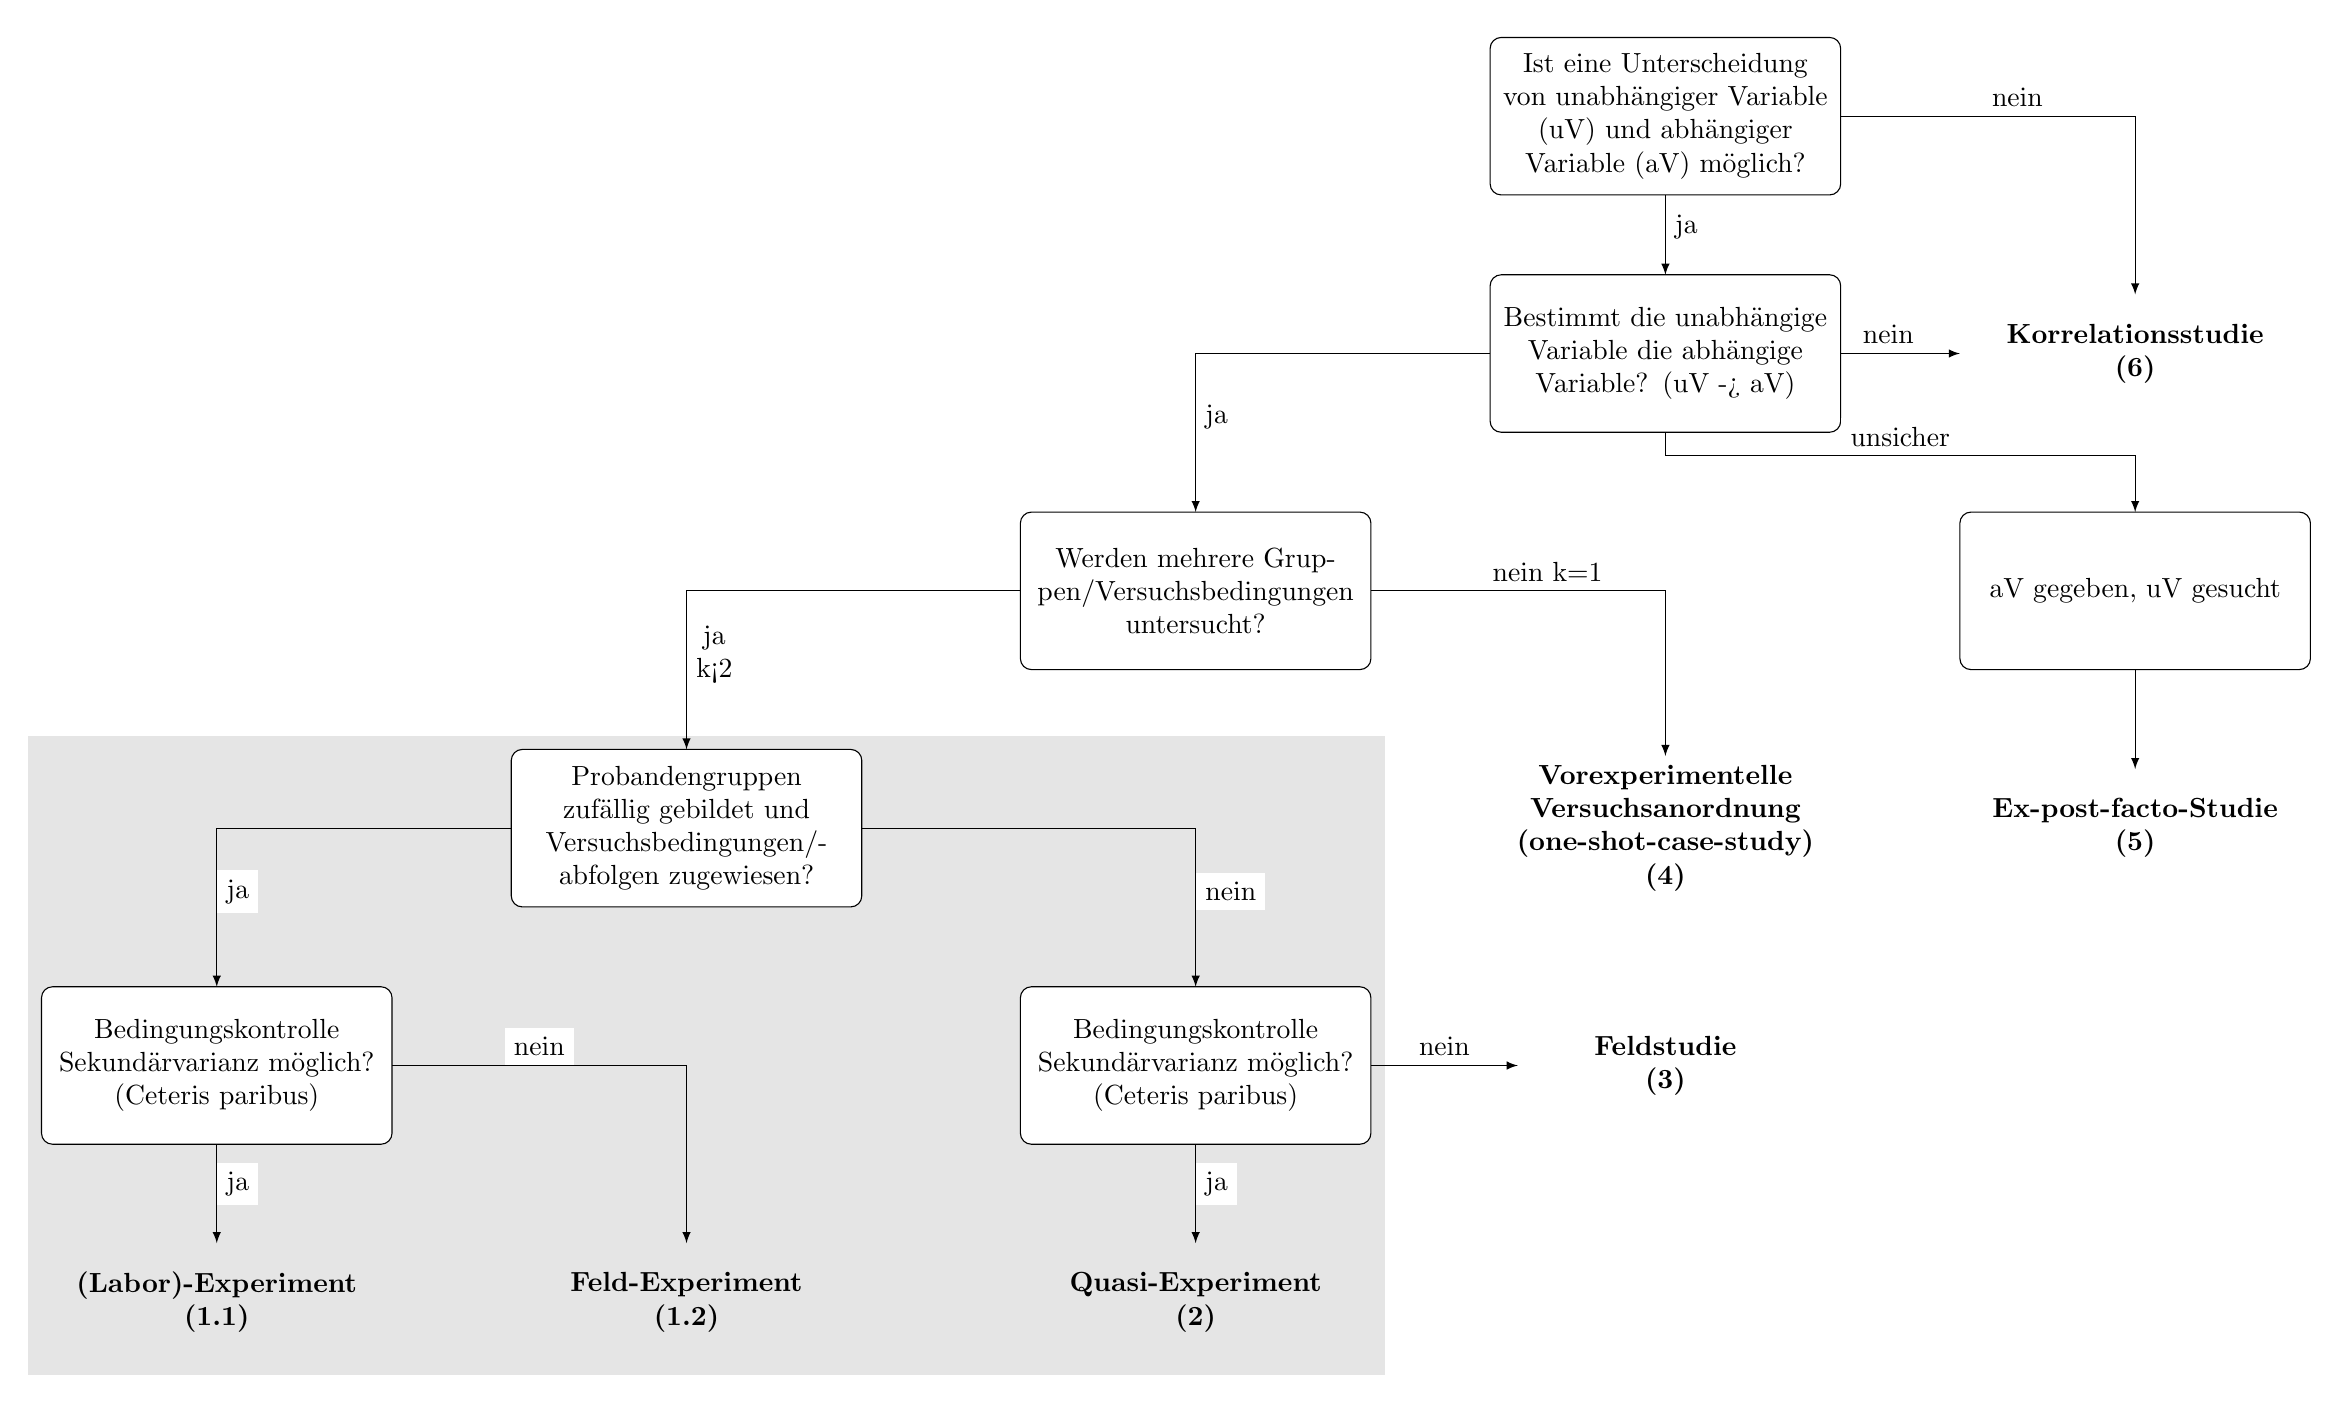
\begin{tikzpicture}
[auto,
decision/.style={diamond, draw=blue, thick, fill=blue!20,text width=4.5em,align=flush center,inner sep=1pt},
block/.style ={ rectangle, draw, fill=white,  text centered, minimum height=15mm, text width=12em},
block_todo/.style ={ rectangle, draw, fill=white,  text centered, minimum height=15mm, text width=12em, rounded corners, outer sep=5},
block_done/.style ={ rectangle, draw, fill=white,  text centered, minimum height=15mm, text width=12em, rounded corners, outer sep=5},
block_normal/.style ={ rectangle, draw, fill=white,  text centered, minimum height=2cm, text width=12em, rounded corners, outer sep=0},
block_exp/.style ={ rectangle, draw=none, fill=none,  text centered, minimum height=1.5cm, text width=12em,font=\bfseries, rounded corners, outer sep=0},
block_phantom/.style ={ block_normal, draw=none, fill=none},
block_background/.style ={ rectangle,  draw=none, fill=black,  text centered, minimum height=15mm,fill opacity=.1, rounded corners=0, inner sep=5},
output/.style ={trapezium,draw,fill=none, minimum height=10mm,  align=center, trapezium left angle=60, trapezium right angle=120, text width=50},
line_inner/.style ={draw, -latex,shorten >=0pt, shorten <=0pt},
kreis/.style ={ circle, draw, fill=white,  text centered, minimum height=15mm, text width=10em, rounded corners, outer sep=0, minimum size=.4cm},
zylinder/.style={cylinder, draw, fill=yellow!20,shape border rotate=90, text height=5, align=center, aspect=.1, text width=10em, minimum height=6.5em, minimum width=2em},
line_outer/.style ={draw, -latex,shorten >=4pt, shorten <=4pt}]
]


\matrix (table) [column sep=1.5cm,row sep=1cm, ampersand replacement=\&,  nodes in empty cells, in front of path]
{
% row 1
\node [block_phantom] (11) {};  \& [0cm]
\node [block_phantom] (12) {}; \& [.5cm]
\node [block_phantom] (13) {};\&
\node [block_normal] (14) {Ist eine Unterscheidung von unabh\"angiger Variable (uV) und abh\"angiger Variable (aV) m\"oglich?};\&
\node [block_phantom] (15) {};\\
 % row 2
\node [block_phantom] (21) {};\& 
\node [block_phantom] (22) {}; \&
\node [block_phantom] (23) {};\&
\node [block_normal] (24) {Bestimmt die unabh\"angige Variable die abh\"angige Variable? (uV -> aV)};\&
\node [block_exp] (25) {Korrelationsstudie \\(6)}; \\
 % row 3
\node [block_phantom] (31) {};\& 
\node [block_phantom] (32) {}; \&
\node [block_normal] (33) {Werden mehrere Gruppen/Versuchsbedingungen untersucht?};\&
\node [block_phantom] (34) {};\&
\node [block_normal] (35) {aV gegeben, uV gesucht}; 
  \\
 % row 4
\node [block_phantom] (41) {};\& 
\node [block_normal] (42) {Probandengruppen zuf\"allig gebildet  und  Versuchsbedingungen/-abfolgen zugewiesen?}; \&
\node [block_phantom] (43) {};\&
\node [block_exp] (44) {Vorexperimentelle Versuchsanordnung (one-shot-case-study)\\(4)};\&
\node [block_exp] (45) {Ex-post-facto-Studie\\(5)};  
   \\
 % row 5
\node [block_normal] (51) {Bedingungskontrolle Sekund\"arvarianz m\"oglich? (Ceteris paribus)};\& 
\node [block_phantom] (52) {}; \&
\node [block_normal] (53) {Bedingungskontrolle Sekund\"arvarianz m\"oglich? (Ceteris paribus)};\&
\node [block_exp,text width=10em] (54) {Feldstudie \\(3)};\&
\node [block_phantom] (55) {}; \\
  % row 6
\node [block_exp] (61) {(Labor)-Experiment\\(1.1)};\& 
\node [block_exp] (62) {Feld-Experiment\\(1.2)}; \&
\node [block_exp] (63) {Quasi-Experiment\\(2)};\&
\node [block_phantom] (64) {};\&
\node [block_phantom] (65) {}; \\
};

%%Pfeile%%%
\draw[line_inner] (14.south) -|  ++(0,0) -|  node[pos=.7, fill=white, rotate=0, align=center] {ja}(24.north);
\draw[line_inner] (24.west) -|  ++(0,0) -|  node[pos=.7,fill=white , rotate=0, align=center] {ja}(33.north);
\draw[line_inner] (33.west) -|  ++(0,0) -|  node[fill=white, pos=.7, rotate=0, align=center] {ja\\k<2}(42.north);
\draw[line_inner] (42.west) -|  ++(0,0) -|  node[fill=white, pos=.7, rotate=0, align=center] {ja}(51.north);
\draw[line_inner] (51.east) -|  ++(0,0) -|  node[fill=white, pos=.25, rotate=0, align=center] {nein}(62.north);
\draw[line_inner] (51.south) -|  ++(0,0) -|  node[fill=white, pos=.7, rotate=0, align=center] {ja}(61.north);
\draw[line_inner] (53.south) -|  ++(0,0) -|  node[fill=white, pos=.7, rotate=0, align=center] {ja}(63.north);
\draw[line_inner] (42.east) -|  ++(0,0) -|  node[fill=white, pos=.7, rotate=0, align=center] {nein}(53.north);
\draw[line_inner] (33.east) -|  ++(0,0) -|  node[fill=white, pos=.3, rotate=0, align=center] {nein k=1}(44.north);
\draw[line_inner] (53.east) -|  ++(0,0) |-  node[fill=white, pos=.75, rotate=0, align=center] {nein}(54.west);
\draw[line_inner] (14.east) -|  ++(0,0) -|  node[fill=white, pos=.3, rotate=0, align=center] {nein}(25.north);
\draw[line_inner] (24.east) -|  ++(0,0) |-  node[fill=white, pos=.7, rotate=0, align=center] {nein}(25.west);
\draw[line_inner] (24.south) -|  ++(0,-.3) -|  node[fill=white, pos=.25, rotate=0, align=center] {unsicher}(35.north);
\draw[line_inner] (35.south) -|  ++(0,-.4) -|  node[ pos=.3, rotate=0, align=center] {}(45.north);

%%%Background%%%%
\begin{scope}[on background layer]
\node[fit=(41)(63), block_background]{};
\end{scope}
%%%Background%%%%


\end{tikzpicture}%
}%
\end{document}%